\section{Background}
\label{sec:rw}

\subsection{Distributed Stream Processing Systems}

Today's de facto programming solution for programming over
distributed streams
is found in \emph{distributed stream processing systems (DSPS)}.
Popular DSPS include
Apache Flink~\cite{Flink,Flink2015},
Timely Dataflow~\cite{Timely,Naiad2013},
and Apache Spark Streaming~\cite{SparkStreaming,Spark2013}.
A selection of these and other systems is included in Table~\ref{fig:dsps-examples}.

To understand the emergence of DSPS and why traditional software infrastructure
is not sufficient, note that traditional software
is often based on the assumption that
critical data can be stored and then processed later.
For example,
much of large-scale data analytics relies on processing data in large
\emph{batches} (e.g. training a machine learning model daily),
such as via MapReduce jobs~\cite{dean2008mapreduce}.
While batch processing
does take advantage of distributed computing resources,
it does not take advantage of the transient and temporal structure of data.
Data is not transient because it must be stored first,
which introduces costs due to batch sizes and data movement.
In practice due to these costs, most data traveling over the internet
and processed by cloud services is either not stored or not harvested to its full potential.
Additionally, the temporal structure of data is lost in batches, which divide
data at arbitrary boundaries in time.
For example, a machine learning model that might benefit from continuous updates is instead trained only on the data from yesterday.
The clear solution to these challenges is to write programs that compute over data in real time.
DSPS offer a software framework for writing such programs, where data processing logic is defined in a platform-independent manner,
then deployed as a distributed application over many nodes.
DSPS performance is measured in terms of \emph{latency} and \emph{throughput};
concretely, stream processing platforms aim for latency in the milliseconds and throughput in tens of thousands of events per process per node.

Despite their popularity and high performance,
programming in DSPS remains difficult for end users.
This has been investigated by software engineering researchers
and surveys~\cite{gulzar2016bigdebug,fisher2012interactions,vianna2019exploratory},
and many of the identified challenges are specific to the big data setting.
For instance, the scale of data makes it difficult to identify faults due to behavior on a single input tuple.
Another source of bugs is that
automatic distribution of stream processing applications
is unfortunately not semantics-preserving~\cite{xiao2014nondeterminism,schneider2013safe,hirzel2014catalog},
which results in nondeterminism due to ordering of distributed events.
Such nondeterminism can lead to bugs that are difficult to identify and reproduce.
In practice, these challenges are partially addressed by rigorous testing, data validation, and offloading of key functionality such as reliable storage to external services, but it would be preferable for DSPS systems to provide more robust behavior in the first place.
In more detail, the following are some of the biggest programming concerns in today's DSPS applications:

\begin{itemize}
\item \emph{Lack of semantics.}
There exists no widely accepted common semantics for distributed stream processing.
DSPS applications are always written as dataflow graphs, and there are other common elements,
but beyond this different APIs make different choices.
For example, Flink's API
assumes that data arrives in-order per-key, whereas Timely's API does not offer this guarantee.
Specific constructs then come with other differences, for example: whether watermarks (indicating stream progress) are explicitly available or implicit;
and
whether side effects are allowed in an operator or whether the system makes no guarantees in the presence of side effects.

\item \emph{Nondeterminism due to event ordering.}
DSPS applications achieve parallelism through \emph{sharding}, which means that operators in the dataflow graph are replicated, and each replica (or shard) processes a subset of the input stream.
However, partitioning of the input stream and collecting of results introduces
the possibility of data reordering.
In practice, many operators are not affected by such reordering: e.g.,
commutative, associative reduce operations or stateless maps and filters.
However in cases where ordering matters,
subtle bugs arise that are not visible at the application level.

\item \emph{Low-level state management.}
DSPS applications are built under the assumption that users should not have to
write state management logic on their own, intsead relying on predefined
dataflow operators (e.g. maps, filters, aggregation, windowing, and SQL query libraries).
In practice, however, some streaming operations require custom logic.
Examples of more complex logic include linear interpolation (fill in missing input data in a temporally dependent manner),
machine learning operators (aggregate and update a statistical model),
and event-dependent windows (form a window with data-dependent start and closing times).
Because of the ubiquity of such manual state management tasks,
popular APIs (including Storm, Flink, and Timely) allow users to program
operators manually, e.g. providing a state type, an initial state, and an
update function for each input tuple.
However, such operators are difficult to program because they must work under
the sharding mentioned above.
Additionally, if the operator requires interaction with an external service or has side effects (e.g. querying a database), state update logic has to be tolerant to unexpected behavior in case of node failures or network communication; yet in practice, users simply ignore these concerns and this results in applications that may crash unexpectedly on a failure.
As a result of these concerns, DSPS developers and researchers generally agree
that better high-level query constructs are needed that alleviate the need for low-level programming.

\item \emph{Manual parallel programming.}
Related to low-level state management, DSPS also promise a programming framework
where users should not have to parallelize their application themselves.
However, in practice, many applications are highly difficult to parallelize and require low-level constructs: for example, a \emph{broadcast} construct is used to broadcast important shared or global state to other nodes.
Such parallel programming is highly prone to correctness bugs.

\item \emph{Unpredictable performance.}
Because operators and input data are partitioned by the system, users
do not describe explicitly how to partition them.
However, DSPS do not offer any concrete guarantees about the throughput or latency of the runtime.
In particular, unexpected performance bugs arise in the
case that partitioning is not efficient.
For instance, in an example application processing
an input stream of webpage views, if most of the views come from the same website,
partitioning by key fails and results in a performance bottleneck.
To address these bugs requires that we have more reliable performance guarantees.
Ideally, application performance could be estimated statically or in conjunction with runtime profiling.
\end{itemize}

\begin{table}[tp]
\begin{Tabular}[3.5]{C{4.5cm}|C{1.4cm}C{1.4cm}C{1.4cm}C{3cm}}
    System & Year & Stable Release & Active? & \makecell{Questions on \\ StackOverflow \\ (as of 2021-04-29)} \\
    \hline
    Aurora
        & 2003~\cite{Aurora} & 2003~\cite{AuroraWeb} & \RedNo{} & -- \\
    Borealis
        & 2005~\cite{Borealis} & 2008~\cite{BorealisWeb} & \RedNo{} & -- \\
    
\includegraphics[align=c,width=0.8\linewidth]{img/systems/storm.png}
        & 2011~\cite{StormInitRelease} & 2020~\cite{Storm} & \GreenYes{} & 2548 \\
    \rule{0pt}{11ex} % some extra spacing here
    \makecell{
    
\includegraphics[align=c,width=0.6\linewidth]{img/systems/flink.png} \\ \cite{Flink,Flink2015}}
        & 2011 & 2021 & \GreenYes{} & 5345 \\
    Google MillWheel
        & 2013~\cite{MillWheel} & -- & \RedNo{} & -- \\
    
\includegraphics[align=c,width=0.8\linewidth]{img/systems/spark.jpg}
    (Apache Spark Streaming)
        & 2013~\cite{Spark2013} & 2021~\cite{SparkStreaming} & \GreenYes{} & 5222 \\
    \makecell{
\includegraphics[align=c,width=0.8\linewidth]{img/systems/samza.png} \\ \cite{Samza,Samza2017}}
        & 2013 & 2021 & \GreenYes{} & 85 \\
    % 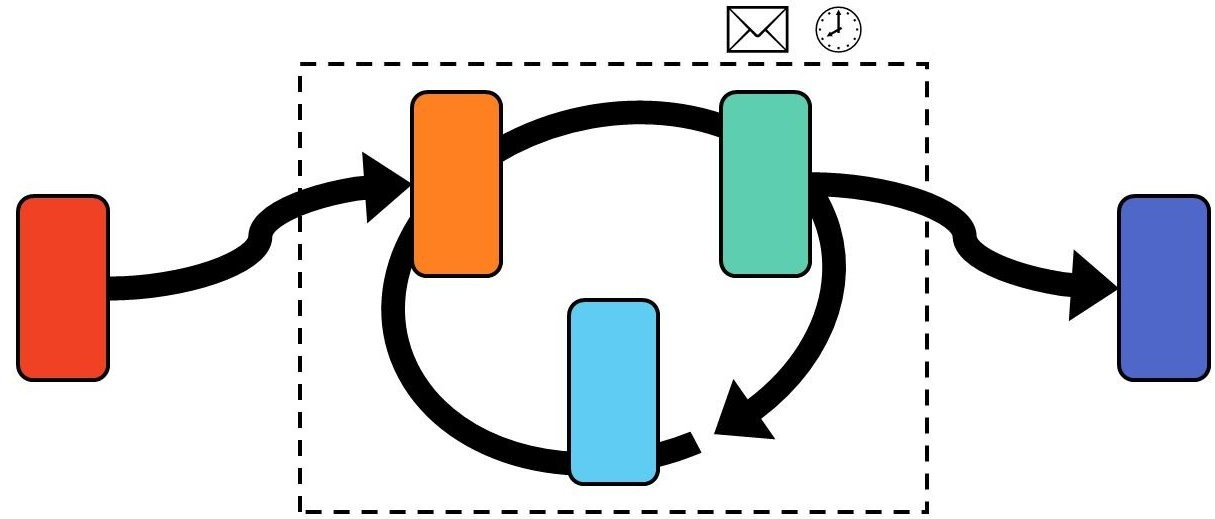
\includegraphics[align=c,width=\linewidth]{img/systems/naiad.jpg}
    Timely Dataflow & 2013~\cite{Naiad2013}
        & 2021~\cite{Timely} & \GreenYes{} & -- \\
    \makecell{
\includegraphics[align=c,width=0.8\linewidth]{img/systems/heron.png} \\ \cite{Heron,kulkarni2015twitter-heron}}
        & 2015 & 2021 & \GreenYes{} & 41 \\
\end{Tabular}

\vspace{0.5cm}

\caption{A selection of major distributed stream processing systems.}
\label{fig:dsps-examples}
\end{table}
